\documentclass{article}
\usepackage[utf8]{inputenc}
\usepackage{graphicx}
\usepackage{hyperref}
\usepackage{amsmath}
\usepackage{fancyhdr}
\pagestyle{fancy}

\fancyhead[LE,RO]{Jesse Both}
\fancyhead[LO,RE]{}


\hypersetup{
    colorlinks = true,
    citecolor=black,
    filecolor=black,
    linkcolor=black,
    urlcolor=blue
}
\graphicspath{ {/graphics/} }
\title{\Huge{\textbf{CSE 454}  \\* Project 2 \\~\\ \textbf{Time Series}}}

\date{} %remove date from make title


%image

% \begin{center}
% {\includegraphics[height=10cm]{*.png}\centering}
% end{center}

\begin{document}
    \maketitle
    \vfill 
    {\Large\centering\textbf{Jesse Both  \\~\\}\par}

    {\Large\centering{Fall 2021}\par}
    {\large\centering{\today}\par}

    \newpage
    \begin{center}
        \tableofcontents
    \end{center}
\newpage
\setcounter{secnumdepth}{-1}


\section{Introduction}
The purpose of this assignment was to explore representation and classification
techniques of a time series.  The data that was used for this assignment was
a \href{https://archive.ics.uci.edu/ml/datasets/Synthetic+Control+Chart+Time+Series}{synthetic control data set}.
The representation techniques that were used for this assignment were PAA - Piecewise
Aggregate Approximation and SAX - Symbolic Aggregate Approximation. The classification
was done by utilizing the Euclidean and Manhattan distance formulas.
\newline
\newline
\noindent
The Euclidean Distance Formula:
$d\left( r,s\right)   = \sqrt {\sum _{i=1}^{n}  \left( r_{i}-s_{i}\right)^2 } $

\noindent
The Manhattan Distance Formula:
$d\left( r,s\right)   = {\sum _{i=1}^{n}  \lvert r_{i}-s_{i}\rvert} $



\section{Data}
The provided data contains 6 classes.  Each sample is contained within 1
row and has 60 columns.  There are 100 samples of each type of class. 
The types of classes include:
\begin{itemize}
    \item Normal
    \item Cyclic
    \item Increasing Trend
    \item Decreasing Trend
    \item Upward Shift
    \item Downward Shift
  \end{itemize}
The class changes after 100 consecutive samples, so the first 100 samples 
are within the normal class followed by the next 100 sample being cyclic.

\subsection{Preprocessing}

In order to get the data into a more usable state, the entire data set was
normalized using MATLAB's normalize() function.  This enables the data to 
be more uniform as well as decreasing the distance between the upper and 
lower bounds.

\subsection{Training Data}
To create a training data set, each class was separated into their own vectors.
Each column was then averaged to find the ideal sample based on the data.  Once 
this was complete the training data would consist of a 6x60 matrix, 1 averaged
row for each class.

\subsection{Testing Data}
The testing data that was used was the original, normalized data set.

\subsection{Data Confusion Matrix}
\begin{center}
    {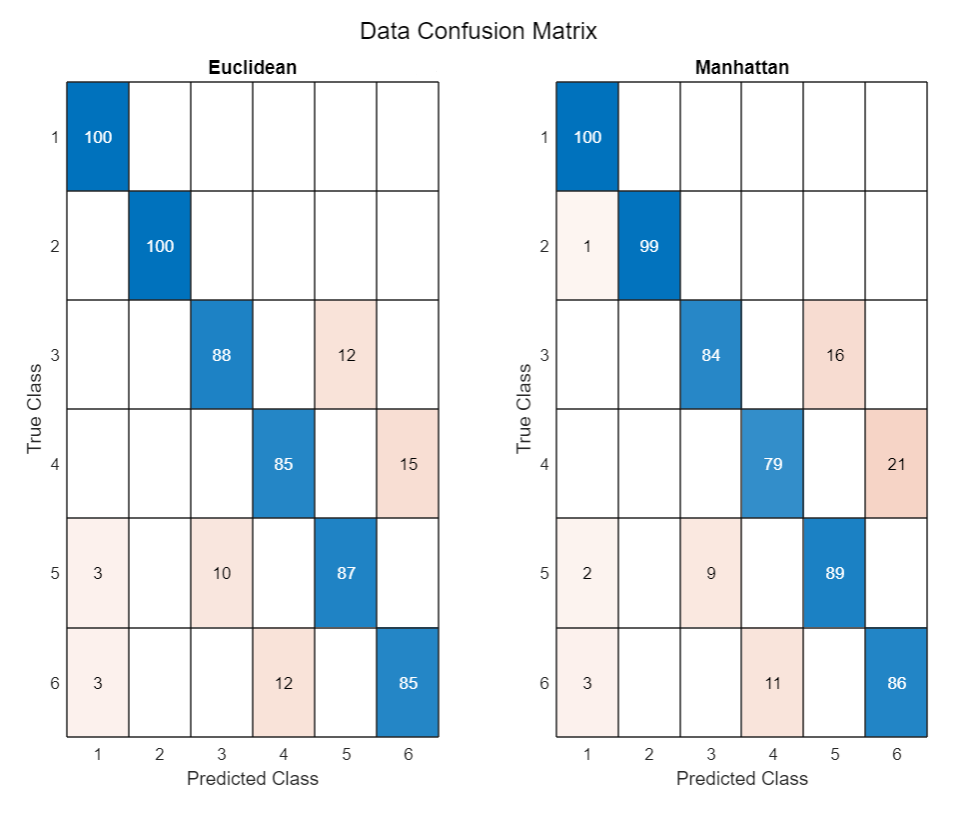
\includegraphics[height=10cm]{graphics/confuseddata.png}\centering}
\end{center}    
It can be seen that there is not much discrepancy between the Euclidean 
and Manhattan formulas, neither is particularly better than the other.
The accuracy rating for the this data using the Euclidean distance formula
is 90.1\% while with the Manhattan formula it is 89.5\%.


\section{PAA}
The implantation that was used was to first determine the size of each window
based on the size of the data set.  The larger the window, the more accurate
the generation will be, but the more processing power would be required to 
utilize the data.  Next, the data is iterated through to determine the upper
or lower bound of each window on the y-axis.  The median of that sample of 
data is then taken to determine the output data point.
\newline
\noindent
The output plot of the data set for each class can be seen below:
\begin{center}
{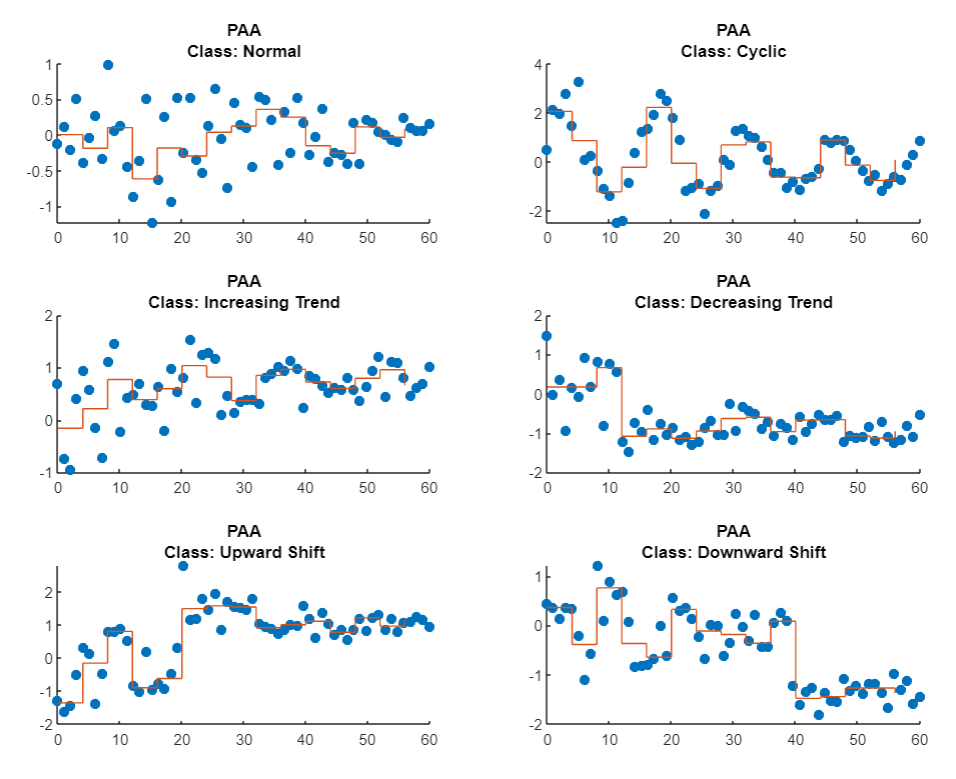
\includegraphics[height=10cm]{graphics/paaplot.png}\centering}
\end{center}

Based on the figure, it can be seen that the PAA generation tries to follow
the data points as best as possible.  It is impossible to have a 100\% accuracy 
rating, but the purpose of these representations is to get as close as possible.
The accuracy rating for the original data using the Euclidean distance formula
is 90.1\% while the PAA generation is 88.7\% with a window size (c) of 15.  With the Manhattan formula, 
the raw data has a 89.5\% accuracy, and with the PAA generation is also
89.5\%
\newline

The spread of the data can be seen in the following matrices.
\begin{center}
    {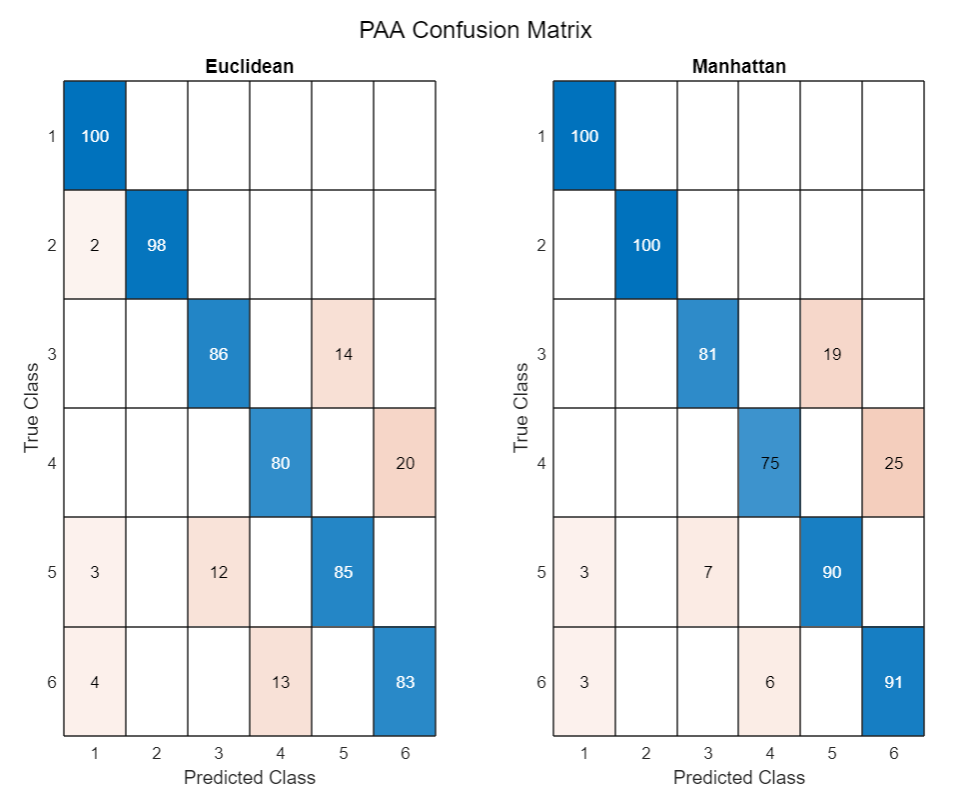
\includegraphics[height=10cm]{graphics/confusedpaa.png}\centering}
\end{center}


\section{SAX}
The process to create the SAX was similar to implementing the PAA, except there
was an additional element that needed to be considered, the labels.  In order to
determine the labels, the ranges of the bounds for each label needs to be defined.
For this implantation, it was chosen that for every value that could be rounded 
to the nearest .5 (of the normalized data) would be its own label.  The labels
that were picked were A-M, A starting at -3 and M ending at +3. 

\begin{center}
    {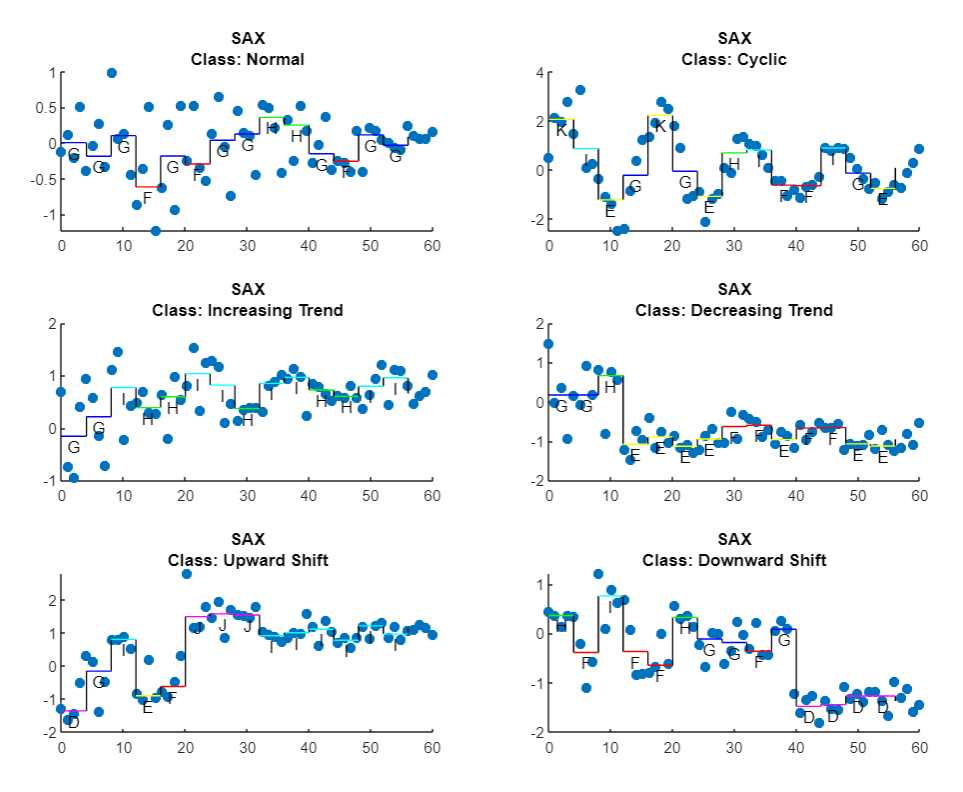
\includegraphics[height=10cm]{graphics/saxplot.png}\centering}
\end{center}

It can be seen in the figures above that when the horizonal lines are close 
enough vertically with each other they are given the same label.

\section{Conclusion}
The PAA and SAX techniques can be utilized to reduce the number of data points 
in a data set.  This allows less processing power to be required in order to use
the data set for practical purposes.
\newline
\noindent
Classification techniques were also explored to compare the accuracy of the data
and the PAA generation.  It can clearly be seen that the reduction in accuracy 
is quite small and does not significantly change the data.


\end{document}
